\chapter{Algorithms}
\label{ch:algorithms}

This chapter briefly explains the different algorithms used in this work. How they are used and what their purpose is for this thesis will be explained in chapter \ref{ch:impl_eval}.\\
All the algorithms are part of a family of algorithms that can be viewed as \emph{machine learning} (ML). In stead of telling a computer what to do to perform a specific task by using explicit instructions, they rely on patterns and inference instead and learn the correct behavior. ML is traditionally divided into 3 subcategories:
\begin{itemize}
    \item \emph{Supervised learning}, where we feed the algorithm with both the input and the correct output so that it can learn based on the predicted and correct output,
    \item \emph{Unsupervised learning}, where the algorithms learns to classify items based on their underlying distribution alone (and thus without being given the correct answer),
    \item \emph{Reinforcement learning} which will be explored in some detail in section \ref{sec:intro_rl}
\end{itemize}


%----------------------------------------------------------------------------
\begin{comment}
\section{Monte-Carlo Tree Search}
\label{sec:intro_mcts}
Monte-Carlo Tree Search (MCTS) \cite{coulom2006efficient} is a heuristic method to efficiently traverse game trees. It is an alternative to more traditional algorithms like \emph{minimax}\cite{russell2016artificial} search that suffer from combinatorial explosion when the game tree becomes too large (both in depth and breadth).\\

The MCTS search process consists of 4 phases:
\begin{enumerate}
    \item \emph{Selection}: starting from a root node $R$, successive child nodes are selected until a \emph{leaf node} $L$ is reached. A leaf node is a node from which no simulation has been done. 
    \item \emph{Expansion}: If node $L$ isn't a terminal node (i.e. the game doesn't reach a terminal state in this node), the different child nodes of $L$ are developed and initiated. A random child node $C$ is chosen among all new child nodes.
    \item \emph{Simulation}: At node $C$ a random simulation is performed. This means that from this node, a sequence of actions is chosen in a uniform random way until a terminal state is reached. 
    \item \emph{Backpropagation}: The result of the simulation (the \emph{reward}) is then used to update the state information of the different nodes that were traversed.
\end{enumerate}

The difficulty in selecting child nodes is maintaining an equilibrium between \emph{exploration} (how much of the game tree do we search) and \emph{exploitation} (picking the actions with the highest expected return). This is accomplished by assigning an \emph{UCT}\footnote{Upper-Confidence Bound for Tree Search} value to each node. The value for the $i^{th}$ action is computed with the expression
\begin{equation}
    UCT(i) = \frac{r_i}{n_i} + c \sqrt{\frac{\ln N}{n_i}}
\end{equation}
with:
\begin{enumerate}
    \item $r_i$ the total reward over all simulations for the node reached with action $i$
    \item $n_i$ the number of times this move was made during the different selection phases
    \item $N$ the number of times the parent node was visited during selection.
    \item $c$ an exploration parameter (typically $2$).
\end{enumerate}
The left term expresses the expected value of action $i$ while the right term is an upper bound on the variance of this value. This right term decreases as the action is frequently chosen. Eventually, an other action $j$ that is less frequently chosen will take over because it's UCT becomes larger as both $N$ and $n_i$ increase.\\

The entire MCTS algorithm is shown in figure \ref{fig:mcts_algo}. Each iteration updates the available information for the nodes that were selected during that iteration. The number of iterations is limited by the time horizon available for exploration. After that time exceeds, the best action is selected for the starting node of the different iterations.
\begin{figure}[htp]
    \centering
    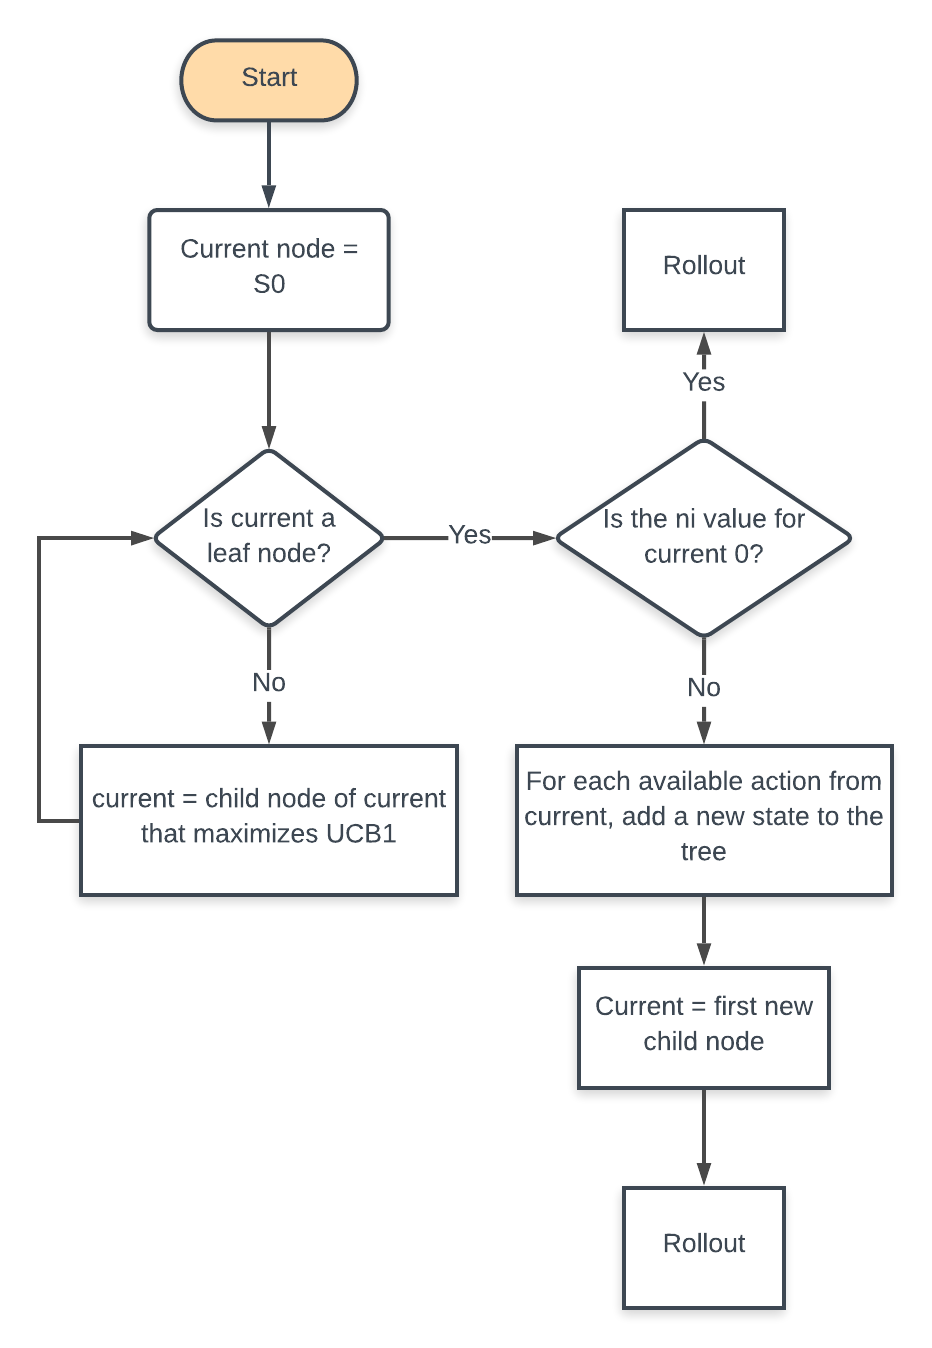
\includegraphics[width=8cm]{images/mcts_algo.png}
    \caption{The MCTS process flow}
    \label{fig:mcts_algo}
\end{figure}

%----------------------------------------------------------------------------
\subsection{MCTS for two-player games}
The previous section describes how MCTS can be used for a single player while traversing a game tree. The question remains how this MCTS player should anticipate which moves his opponent will make while selecting nodes in search for a leaf node. The most obvious way of doing this is working with a turn-based game and simultaneously training another MCTS player on this game. We can then use the game play of the other player to simulate the opponent. 

\begin{figure}[htp]
    \centering
    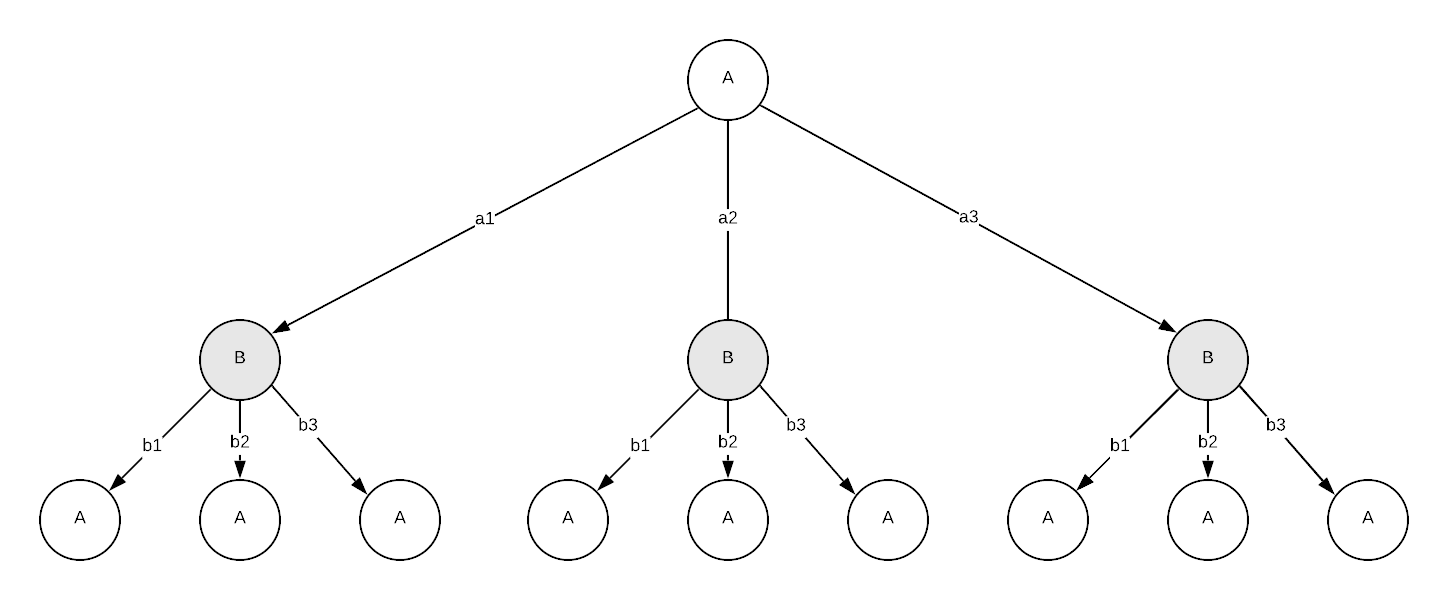
\includegraphics[width=10cm]{images/game_tree.png}
    \caption{Game tree for a two-player turn based game}
    \label{fig:game_tree}
\end{figure}
\end{comment}
%----------------------------------------------------------------------------
\section{Reinforcement Learning}
\label{sec:intro_rl}
Reinforcement Learning (RL) is a form of Machine Learning where an agent learns what to do in order to maximize a numerical reward signal \cite{sutton2018reinforcement}. RL uses a \emph{Markov Decision Process} (MDP) as the formal framework to solve a sequential decision making problem. In this framework, the learner and decision maker is the \emph{agent} who interacts with the \emph{environment} at discrete time steps $t=0, 1, 2, \ldots$. At each time step $t$, the agent receives a representation of the environment's \emph{state} $S_t$\footnote{A note on notation: when we want to represent a generic state, action or reward, a lower case letter will be used ($r$, $a$, $r$). When we refer to a specific instance, e.g. obtained through sampling, we use capital letters ($S_t$, $A_t$, $R_t$) with an index that refers to the time instant when this sample was generated.}. Based on this state information, the agent decides which action $A_t$ to take and sends this action to the environment. The environment changes its internal state to a new state $S_{t+1}$ and sends a reward signal $R_{t+1} \in \mathbb{R}$ back to the agent. This reward gives an indication how good the chosen action was. The Markov decision process is represented in figure \ref{fig:mdp}.\\


\begin{figure}[htp]
    \centering
    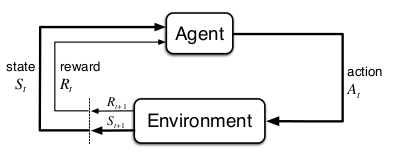
\includegraphics[width=8cm]{images/mdp.png}
    \caption{The agent-environment interface of an MDP (reproduced from \cite{sutton2018reinforcement})}
    \label{fig:mdp}
\end{figure}

The goal of RL is to choose a sequence of actions that maximizes the \emph{cumulative discounted reward} $G_t$:
\begin{equation}
\begin{split}
    G_t &= \sum_{k=0}^{\infty} \gamma^k R_{t+k+1} \\
        &= R_{t+1} + \gamma G_{t+1}
\end{split}
\label{eqn:cum_reward}
\end{equation}
where $0 \leqslant \gamma \leqslant 1$ is the \emph{discount factor}.\\

A function $\pi(s)$ is called a \emph{policy} when it returns an action $a$ to take in state $s$. More generally, a policy can also return a probability distribution over actions. In that case it is denoted as $\pi(a|s)$ (read: the policy over actions $a$ given that we are in state $s$).\\

The \emph{value} of a policy $V_{\pi}$ is the expected value of $G_t$ when starting in state $S_t=s$ and following policy $\pi$:
\begin{equation}
    V_{\pi}(s) = \mathbb{E_{\pi}}[G_t | S_t=s]
     \label{eq:definition_V}
\end{equation}
The expected value of taking action $a$ in state $s$ under policy $\pi$ is denoted as $Q_{\pi}(s,a)$ and is called the \emph{action-value function for $\pi$}:
\begin{equation}
    Q_{\pi}(s,a) = \mathbb{E_{\pi}}[G_t | S_t=s, A_t = a]
    \label{eq:definition_Q}
\end{equation}

When a policy maximizes equation \ref{eqn:cum_reward} it is called the optimal policy $\pi_{*}$ and one can show that action-value function $Q_{*}(s, a)$ of this optimal policy obeys a recursive relationship called the \emph{Bellman optimality equation}:
\begin{equation}
    Q_{*}(s,a) = \sum_{s', r} p(s', r | s, a) \big[r + \gamma \max_{a'} Q_{*}(s', a') \big]
    \label{eqn:bellman}
\end{equation}
with $p(s', r | s, a)$ the probability of receiving reward $r$ and moving to state $s'$ if being in state $s$ and taking action $a$. When $Q_{*}(s,a)$ is known, the optimal policy can be trivially computed with:
\begin{equation}
    \pi_{*}(s) = \argmax_{a} Q_{*}(s, a)
    \label{eq:optimal_policy}
\end{equation}

Several classical algorithms exist to solve this problem. However, they all assume that the state-transition probabilities $p(s', r | s, a)$ are known. Typically this is not the case and these probabilities have to be estimated. Methods that have no model of the transition probabilities are called \emph{model-free}. These models learn from by interacting with the environment by creating \emph{trajectories} of successive states, actions and rewards:
$$
\ldots, S_{t-1}, A_{t-1}, R_t, S_t, A_t, R_{t+1}, S_{t+1}, \ldots
$$
\\
The goal of RL is to learn the optimal policy $\pi_{*}(s)$. To accomplish this, two paradigms exist: value approximation, where we first approximate $Q(s,a)$ and then derive the policy according to \ref{eq:optimal_policy}, and policy approximation, where we derive the optimal policy $\pi_{*}(a|s)$ directly. Both a paradigms are explained below.
%----------------------------------------------------------------------------
\subsection{Value approximation: Q-learning}
\label{sec:intro_q_learning}
The most well-known model-free method is \emph{Q-learning} \cite{watkins1989learning}. This iterative algorithm builds on equation \ref{eqn:bellman} to estimate $Q_{*}(s,a)$ by making a step in the direction of the \emph{temporal difference}, the difference between the value estimate $Q(S_t, A_t)$ in the current state and the best value we can obtain from a next state:
\begin{equation}
    Q(S_t, A_t) \leftarrow Q(S_t, A_t) + \alpha \big[R_{t+1} + \gamma \max_{a} Q(S_{t+1}, a) - Q(S_t, A_t) \big]
    \label{eqn:q_learning}
\end{equation}
where $\alpha$ is the step size. The authors of \cite{watkins1992q} show that the empirical estimate $Q(S_t, A_t)$ converges to $Q_{*}(s,a)$.\\

The entire algorithm is shown in algorithm \ref{algo:q_learning}. Note the use of the current estimate $Q$ to select the next action $A$ to take.

\begin{algorithm}[H]
\SetAlgoLined
\textbf{Input}:  step size $\alpha$\\
Initialize $Q(s,a)$ for all $s \in \mathcal{S}$, all $a \in \mathcal{A}$\\
 \For{each episode}{
    \For{each step of the episode}{
        Choose action $A$ from state $S$ using policy derived from $Q$ (e.g. see eqn. \ref{eq:optimal_policy})\\
        Take action $A$, observe reward $R$ and next state $S'$\\
        $Q(S, A) \leftarrow Q(S, A) + \alpha \big[R + \gamma \max_{a} Q(S', a) - Q(S, A) \big]$\\
        $S \leftarrow S'$
  } until $S$ is terminal\\
 }
 \caption{Q-Learning}
 \label{algo:q_learning}
\end{algorithm}

%----------------------------------------------------------------------------
\subsection{Policy approximation: Policy Gradients}
\label{sec:intro_policy_grads}
The value approximation family of RL algorithms estimates the state-action value $Q(s,a)$ and then uses this estimate to select the best available action with equation \ref{eq:optimal_policy}. An other family of algorithms, the \emph{policy gradient} (PG) methods \cite{sutton2000policy}, tries to find the optimal policy directly.\\

For these algorithms, a policy $\pi(a|s)$ is determined by a parameter vector $\bm{\theta} \in \mathbb{R}^d$. The goal of the algorithm is to adjust $\bm{\theta}$ such that it maximizes a certain performance measure $J(\bm{\theta})$. In episodic MDP's, the performance measure will be the value of initial state: $J(\bm{\theta}) = v_{\pi_{\bm{\theta}}}(S_0)$. Maximizing $J(\bm{\theta})$ is typically done taking a step in the direction of the gradient of  $J(\bm{\theta})$ with respect to $\bm{\theta}$, a procedure called \emph{gradient ascent}:
\begin{equation}
    \label{eqn:grad_ascent}
    \bm{\theta}_{t+1} = \bm{\theta}_{t} + \alpha \nabla_{\bm{\theta}} J(\bm{\theta})
\end{equation}
Computing the gradient $\nabla_{\bm{\theta}} J(\bm{\theta})$ is non-trivial in general, but under certain conditions we can use the \emph{policy gradient theorem} which states that:
\begin{equation}
    \begin{split}
    \nabla J(\bm{\theta}) &\propto \sum_{s} \mu(s) \sum_{a} q_{\pi}(s,a) \nabla_{\bm{\theta}} \pi(a|s, \bm{\theta})\\
                          &\propto \mathbb{E}_{\pi} \Big [ G_t \frac{\nabla_{\bm{\theta}} \pi(A_t|S_t, \bm{\theta})}{\pi(A_t|S_t, \bm{\theta})}\Big]
    \end{split}
    \label{eqn:pol_grad_theorem}
\end{equation}
with $\mu(s)$ the distribution of states under policy $\pi$. The last expression is the one based on samples drawn from interacting with the environment. This equation is very useful because it links the gradient of the performance measure $J(\bm{\theta})$ to the gradient of the policy $\pi(A_t|S_t, \bm{\theta})$ which can easily be computed (especially with automatic differentiation frameworks like {\tt PyTorch} - see section \ref{sec:intro_deep_rl}).\\
It follows that the policy parameter vector $\bm{\theta}$ is updated according to following rule:
\begin{equation}
    \bm{\theta} \leftarrow \bm{\theta} + \alpha \, G_t \, \frac{\nabla_{\bm{\theta}} \pi(A_t|S_t, \bm{\theta})}{\pi(A_t|S_t, \bm{\theta})}
    \label{eqn:reinforce_update}
\end{equation}
This expression has intuitive appeal: each increment of $\bm{\theta}$ is in the direction in parameter space that most increases the probability of taking action $A_t$ in state $S_t$. This direction is multiplied by the expected reward $G_t$ and divided by the action probability $\pi(A_t|S_t)$. The former causes the parameter to move most in directions that favor actions with higher returns. The latter makes sense because otherwise actions that are selected frequently have an unfair advantage.

%Derivation of theorem:
%\begin{equation}
%    \begin{split}
%        \nabla_{\theta} E_x[f(x)] &= \nabla_{\theta} \sum_x p(x) f(x) \\
%                                  &= \sum_x \nabla_{\theta} p(x) f(x) \\
%                                  &= \sum_x p(x) \frac{\nabla_{\theta}p(x)}{p(x)} f(x) \\
%                                  &= \sum_x p(x) \nabla_{\theta} \log p(x) f(x) \\
%                                  &= E_x[f(x) \nabla_{\theta} \log p(x)] \\
%    \end{split}
%\end{equation}

Implementing equation \ref{eqn:reinforce_update} directly leads to the simplest PG algorithm, REINFORCE \cite{williams1992reinforce}:

\begin{algorithm}[H]
\SetAlgoLined
\textbf{Input}: A differentiable policy $\pi(a|s, \bm{\theta})$\\
Initialize $\bm{\theta} \in \mathbb{R}^d$\\
 \While{not converged}{
  Generate an episode $S_0, A_0, R_1, \ldots, S_{T-1}, A_{T-1}, R_T$, following $\pi(a|s,\bm{\theta})$ \\
  \For{each step of the episode $t=0, \ldots, T-1$}{
    $G_t \leftarrow$ return from step $t$ \\
    $\bm{\theta} \leftarrow \bm{\theta} + \alpha \, G_t \, \nabla_{\bm{\theta}} \ln \pi(A_t|S_t,\bm{\theta})$
  }
 }
 \caption{REINFORCE}
 \label{algo:reinforce}
\end{algorithm}

Note that $\nabla_{\bm{\theta}} \ln \pi$ is shorthand for $\frac{\nabla_{\bm{\theta}} \pi}{ \pi}$.
%----------------------------------------------------------------------------
\subsection{Actor-Critic Methods}
\label{sec:actor_critic}
While REINFORCE in theory converges to an optimal policy, it suffers from high variance: the gradient estimates are unbiased but very noisy. Thus convergence is slow and the algorithm is very sample-inefficient, i.e. many samples must be generated to achieve an acceptable result. A simple fix would be to add a \emph{baseline} $b(S_t)$ that is then subtracted from the cumulative reward $G_t$. It is important that this baseline only depends on the state and not on the action. If that is the case, the expected value in \ref{eqn:pol_grad_theorem} keeps it's value, namely $\nabla J(\bm{\theta})$ and the estimator remains unbiased. The new update rule then becomes (from \cite{sutton2018reinforcement}):
\begin{equation}
    \label{eqn:pg_update}
    \bm{\theta}_{t+1} = \bm{\theta}_{t} + \alpha \,\big ( G_t - b(S_t) \big) \, \nabla_{\bm{\theta}} \ln \pi(A_t|S_t,\bm{\theta})
\end{equation}

Actor-Critic methods \cite{konda2000actor} are methods that use a parametric policy $\pi(a|s, \bm{\theta})$ (the \emph{actor}) to select actions and a function $\hat V(s|\bm{w})$ (the \emph{critic}) to estimate the value of a state, just as in Q-learning methods. The baseline $b(S_t)$ then becomes the estimated state-value $V(S_t)$. Rewriting equation \ref{eqn:pg_update} leads to:
\begin{equation}
    \label{eqn:actor_critic}
    \begin{split}
    \bm{\theta}_{t+1} &= \bm{\theta}_{t} + \alpha \,\big ( G_t - \hat V(S_t) \big) \,                                       \nabla_{\bm{\theta}} \ln \pi(A_t|S_t,\bm{\theta}) \\
                     &= \bm{\theta}_{t} + \alpha \,\big ( R_{t+1}+\gamma \hat V(S_{t+1}) - \hat V(S_t) \big) \,                                       \nabla_{\bm{\theta}} \ln \pi(A_t|S_t,\bm{\theta}) \\
    \end{split}
\end{equation}
where $G_t$ is replaced by $R_{t+1}+\gamma \hat V(S_{t+1}$ according to equation \ref{eqn:cum_reward}. This is the update rule for the actor; in parallel, the critic is trained to accurately estimate the value of the state $S_t$.\\
\begin{algorithm}[H]
\SetAlgoLined
\textbf{Input}: A differentiable policy $\pi(a|s, \bm{\theta})$ and value-function $V(S, \bm{w})$\\
Initialize $\bm{\theta} \in \mathbb{R}^d$\\
 \While{not converged}{
 Initialize $S$ (first state of the episode)\\
 $I \leftarrow 1$\\
 \While{S is not terminal}{
    Sample $A ~ \pi(a|s,\bm{\theta}) $ \\
    Take action $A$, observe next state $S'$ and reward $R$\\
    $\delta \leftarrow R + \gamma \hat V(S', \bm{w}) - V(S, \bm{w})$\\ % TODO: replace with \mathcal{A}(S_t, A_t) and verify if this is still ok
    $ \bm{w} \leftarrow \bm{w} + \alpha^{\bm{w}} I \delta \nabla_{\bm{w}} \hat V(S, \bm{w})$    ($\rightarrow$ Update rule for the \emph{critic})\\
    $\bm{\theta} \leftarrow \bm{\theta} + \alpha^{\bm{\theta}} I \delta \nabla_{\bm{\theta}} \ln \pi(A_t|S_t,\bm{\theta})$ ($\rightarrow$ Update rule for the \emph{actor}) \\
    $I \leftarrow \gamma I$, $S \leftarrow S'$
  }
 }
 \caption{Actor-Critic Algorithm (from \cite{sutton2018reinforcement})}
 \label{algo:actor_critic}
\end{algorithm}
An alternative is to notice that according to equation \ref{eq:definition_Q}, $Q(s,a)$ is an unbiased estimator for $G_t$. Replacing $G_t$ by $\hat Q(S_t, A_t)$ and using baseline $\hat V(S_t)$ leads to
\begin{equation}
\bm{\theta}_{t+1} = \bm{\theta}_{t} + \alpha \,\big (\hat Q(S_t, A_t) - \hat V(S_t) \big) \, \nabla_{\bm{\theta}} \ln \pi(A_t|S_t,\bm{\theta})
\end{equation}
where the term $Q(s,a) - V(s)$ is also known as the \emph{advantage} $\mathcal{A}(s, a)$ of taking action $a$ in state $s$. $\mathcal{A}(s, a)$ is the improvement (positive or negative) that action $a$ can bring in state $s$ compared to the expected value $V(s)$ of that state. If we use the advantage function, the algorithm is known as $A2C$ which stands for \emph{Advantage Actor-Critic}.\\
\begin{comment}
This method can be further improved by replacing the advantage $\mathcal{A}(S_t, A_t)$ by the \emph{Generalised Advantage Estimation} ${A}_t^{GAE(\gamma, \lambda)}$ \cite{schulman2015high}:
\begin{equation}
    \mathcal{A}_t^{GAE(\gamma, \lambda)} = \sum_{l=0}^{\infty}(\gamma \lambda)^l \delta_{t+l}
\end{equation}
with $\delta_{t+l} = R_{t+1}+\gamma \hat V(S_{t+1}) - \hat V(S_t)$.\\
\end{comment}
Another advantage of the Actor-Critic algorithm in \ref{algo:actor_critic} is that the update of the both estimators can be done after each new sample, while in REINFORCE we must first generate an entire episode before any learning can be done. Notice also that the step sizes for critic and actor (resp. $\alpha^{\bm{w}}$ and $\alpha^{\bm{\theta}}$) are different.\\

%----------------------------------------------------------------------------
\section{Deep Reinforcement Learning}
\label{sec:intro_deep_rl}
The RL algorithms described in the previous section use function approximators to represent the policy $\pi(a|s)$, the value function $V(s)$ or the state-action function $Q(s,a)$. These function approximators are most commonly implemented as neural networks. If that's the case, we speak of \emph{Deep Reinforcement Learning} (DRL). In order to describe these DRL algorithms, we first explain what is \emph{Deep learning} and how it differs from other ML algorithms.

%------------------------------------------------------------------------------------------------------
\subsection{Deep Learning}
\label{sec:deep_learning}

\subsubsection{Neural Networks}
Artificial intelligence in general and machine learning in particular made significant progress with the advent of \emph{Deep Learning} \cite{goodfellow2016deep}. This is nothing more than a collection of methods for designing and training \emph{neural networks} with several layers (hence \emph{deep}). An artificial neural network is a function approximator that mimics the structure of the human brain, albeit in a very coarse way. It consists of layers of artificial neurons - see figure \ref{fig:neuron}. These are mathematical objects that have several inputs $x_1, \ldots, x_m$, each of which are multiplied by a weight $w_i$ and then summed (together with a bias term $b_i$). This sum is then applied to an \emph{activation function} $\phi(\cdot)$ to produce the output:
\begin{equation}
    \begin{split}
    y &= \phi \Big (\sum_{i=1}^{m}w_i x_i + b \Big) \\
      &= \phi (\bm{w}^T \bm{x} + b) 
    \end{split}
\end{equation}

\begin{figure}[htp]
    \centering
    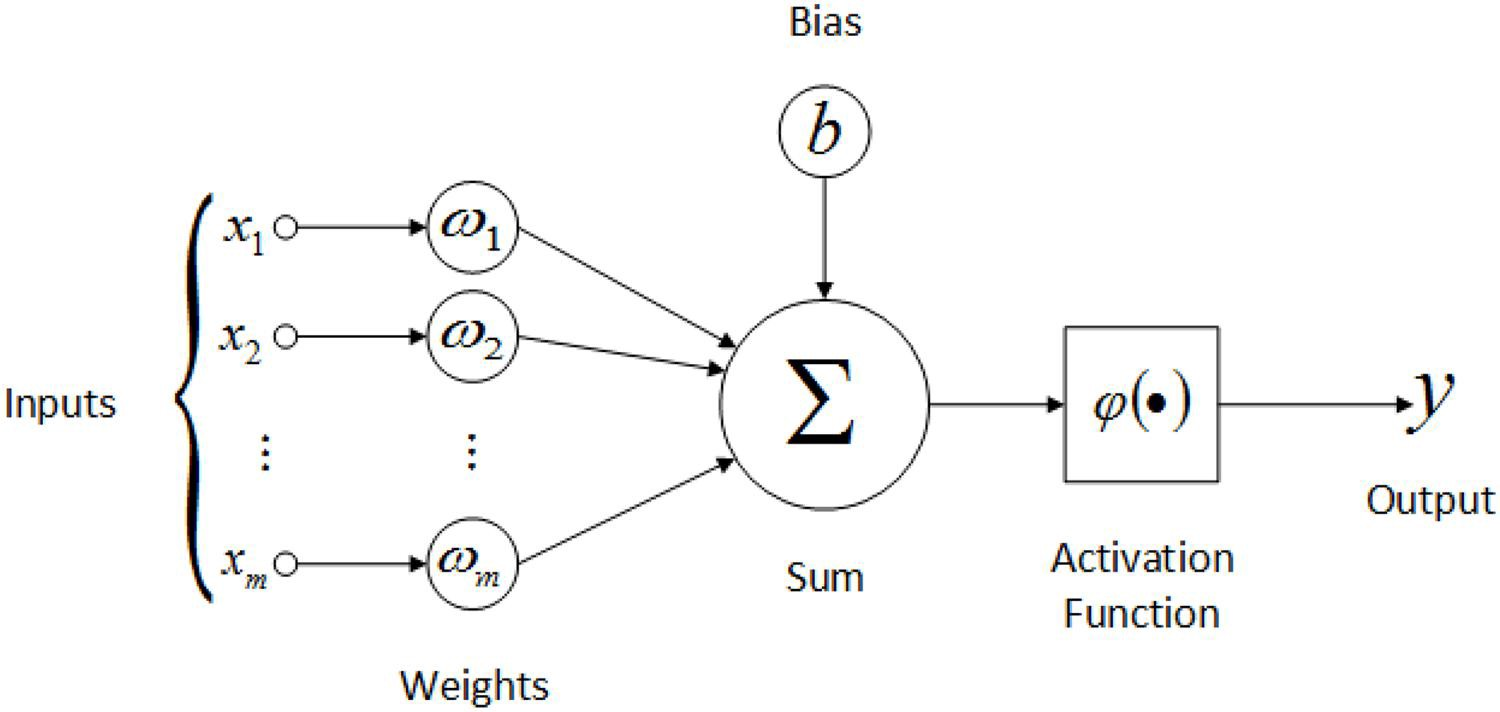
\includegraphics[width=10cm]{images/neuron.jpeg}
    \caption{An artificial neuron}
    \label{fig:neuron}
\end{figure}

The activation function $\phi$ has to be non-linear function like a sigmoid $\sigma(\cdot)$, a hyperbolic tangent function or a rectified linear unit (ReLU). These functions are represented in figure \ref{fig:activation_funcs}. It is important that these functions are non-linear; otherwise, the neural network would have no more representational power than a simple linear function.

\begin{figure}[htp]
    \centering
    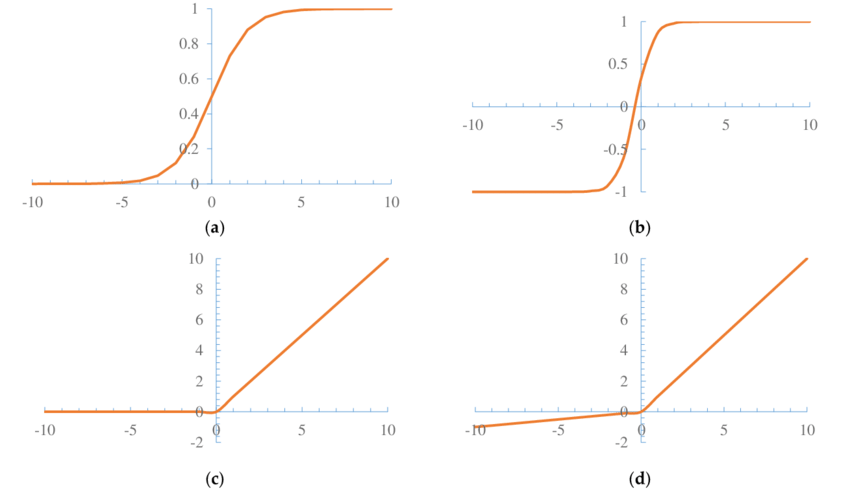
\includegraphics[width=10cm]{images/activation_funcs.png}
    \caption{Activation functions: (a) sigmoid, (b): tanh, (c) ReLU, (d) Leaky ReLU}
    \label{fig:activation_funcs}
\end{figure}

Neural networks \cite{nielsen2015neural} are made of several layers of these artificial neurons (the white dots in figure \ref{fig:neural_net}). In this figure an input of $8$ components is fed to the input layer and propagates through the different layers. At each step, the values are multiplied by the weights and passed through an activation function. Since the network has four output nodes, it can classify the input vector in four categories using one-hot encoding (i.e. for each category, only one output node will be activated while the others stay at zero).
%----------------------------------------------------------------------------
\subsubsection{Stochastic Gradient Descent}
Training this network means adjusting the neuron weights to minimize some error criterion. This is done by feeding samples to the input layer and comparing the produced output with the desired output. The error between both is used to adjust the different weights $w_i$ of the neurons with the help of an algorithm called \emph{backpropagation}. For each training sample we have the corresponding correct output; hence, this procedure is called \emph{supervised learning}.\\

\begin{figure}[htp]
    \centering
    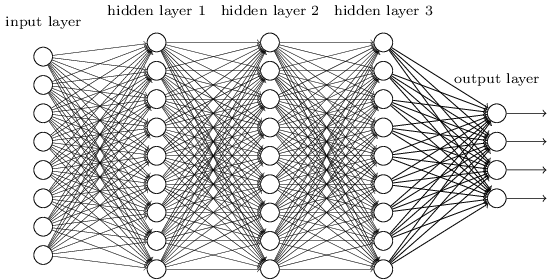
\includegraphics[width=12cm]{images/neural_net.png}
    \caption{A multi-layer neural net (reproduced from \cite{nielsen2015neural})}
    \label{fig:neural_net}
\end{figure}

In order to adjust the network weights, the most commonly used procedure is \emph{stochastic gradient descent}, which is the sample-based variant of expression \ref{eqn:grad_ascent}. In stead of computing the gradient exactly, we estimate it based on one or on a few samples and their corresponding loss $J_{i}(\bm{\theta})$: 
\begin{equation}
    \label{eqn:sgd}
    \bm{\theta}_{t+1} = \bm{\theta}_{t} - \alpha \frac{1}{N} \sum_{i=1}^{N} \nabla_{\bm{\theta}} J_{i}(\bm{\theta})
\end{equation}
with $N$ the number of samples.

While this technique only finds a local rather than a global minimum of the loss function, it has been shown that the resulting optimum works well in practice \cite{bottou2010large}.  However, if the local error surface is not well conditioned (i.e. there is a large difference in eigenvalues of the Hessian), convergence to the local minimum can be slow. A popular method to speed up convergence is SGD with \emph{momentum} \cite{qian1999momentum}, where the gradient that is used for the update is a moving average of the previous immediate gradients:

\begin{align*}
        V_t &= \beta \, V_{t-1} + (1-\beta) \sum_{i=1}^{N} \nabla_{\bm{\theta}} J_{i}(\bm{\theta})\\
        \bm{\theta}_{t+1} &= \bm{\theta}_{t} - \alpha V_t
\end{align*}
with $0 \leq \beta < 1$.\\
A popular implementation of this paradigm is \emph{Adam} \cite{kingma2014adam}, an algorithm that uses momentum with an adaptive step size. This is the optimization algorithm that will be used throughout this thesis.

%----------------------------------------------------------------------------
\subsubsection{Convolutional Neural Networks}
A \emph{Convolutional Neural Network} (CNN) \cite{lecun1989backpropagation} is a specific instance of an artificial neural network where several square windows `glide` over an image and at each position the covered pixels are multiplied by the window weights and summed. This operation is called a \emph{convolution}. These kind of networks are very well suited for processing images since they implicitly capture that the salient characteristics (forms, colors, texture, \ldots) of objects in images are invariant to translations.\\

The typical structure of a CNN used for classification is shown in figure \ref{fig:typical_cnn}. The input is an image of a robot. This image has a height and width (in number of pixels) and three color channels. Several convolutional windows process the image as described above and create a set of \emph{feature maps}. One of these maps might be for example the vertical edges, another the horizontal \ldots. The important thing is that the coefficients of these windows are learned by the system, and not defined by the user. Other elements however, like the size and number of these windows are part of the network architecture and must be defined by the programmer. \\

\begin{figure}[htp]
    \centering
    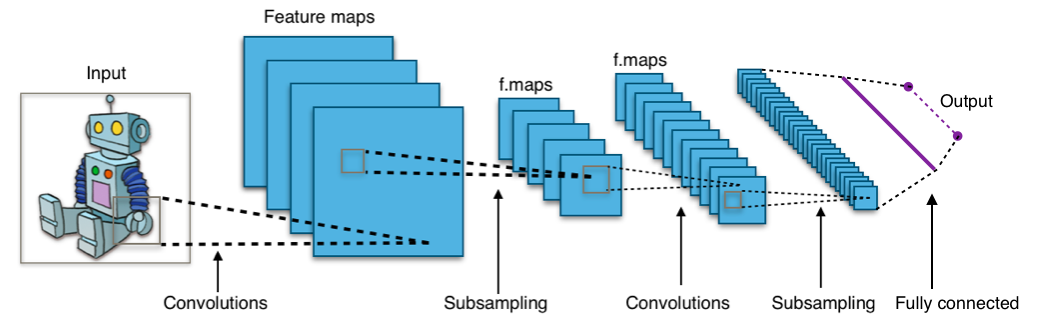
\includegraphics[width=14cm]{images/typical_cnn.png}
    \caption{Structure of a typical CNN}
    \label{fig:typical_cnn}
\end{figure}

After the convolutions typically follows a subsampling phase, where for a window of pixels only the one with the maximum value is retained (\emph{max-pooling}) and which will reduce the computational overhead. Another sequence of convolutions and subsampling leads to a final set of feature maps. The idea is to learn more complex features as we move up in to hierarchy, going form edges to textures to parts of objects to complete objects. These feature maps are then reduced to a single vector which will be processed by a more traditional multi-layer network (a sequence of fully-connected layers).\\

%----------------------------------------------------------------------------
\subsubsection{Recurrent Neural Networks}
Another type of neural network is a \emph{Recurrent Neural Network} (RNN), which is mostly used to model sequential inputs. The output of the network is at the next time step fed back to the input (after multiplication with weights $V$ and activation), as shown in the left image of figure \ref{fig:rnn}. To analyze these kind of networks, they are "unfolded" so that each step is represented by a separate but identical network (the right part of figure \ref{fig:rnn}). The internal state vector $\bm{h}$ (also called the \emph{hidden state}) is then at each time step seen an a new "input" $\bm{h}_t$ to the network at time $t$, just as the true input $\bm{x}_t$.\\
\begin{figure}[htp]
    \centering
    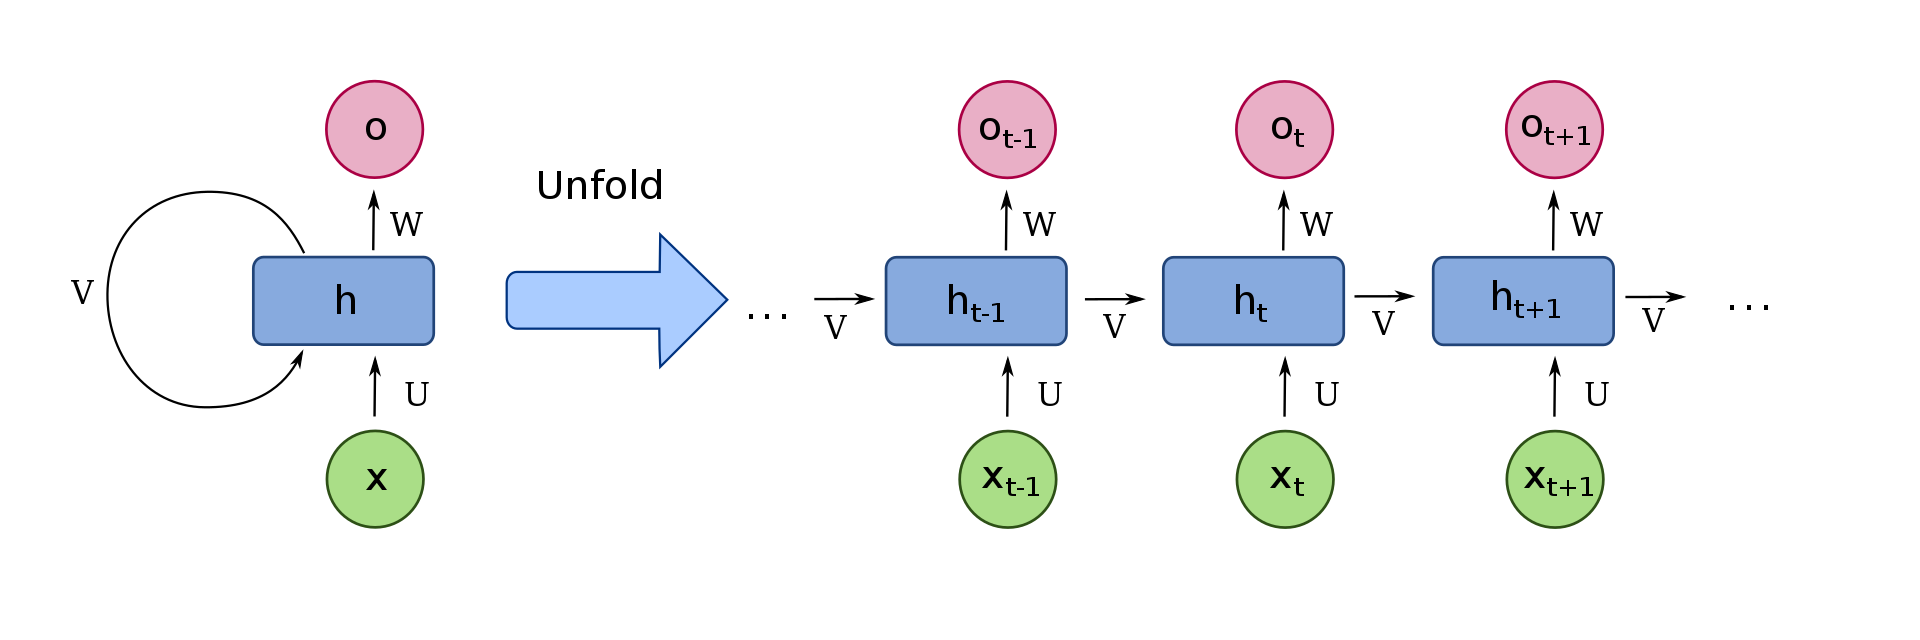
\includegraphics[width=14cm]{images/rnn.png}
    \caption{Structure of a typical RNN}
    \label{fig:rnn}
\end{figure}
The most prominent examples of RNN's are Long Short-Term Memory (LSTM) \cite{hochreiter1997long} networks and Gated Recurrent Unit (GRU) \cite{cho2014learning} networks. These networks extend the basic structure of figure \ref{fig:rnn} to better model long-term dependencies in the input sequence. In what follows, GRU's will be explored in some detail since they will be the neural network of choice to model the policy- and actor networks of the different agents.\\

GRU's use gating mechanisms to control and manage the flow of information between cells in the neural network. The goal is to capture dependencies from large sequences of data without discarding relevant information from earlier parts of the sequence. A GRU cell contains two gates: an \emph{update gate} and a \emph{reset gate} who are trained to selectively filter out any irrelevant information while keeping what is useful. In essence, these gates are vectors containing values between $0$ and $1$ which are multiplied with the input data or the hidden state. A $0$ means this information is unimportant, while a $1$ signifies the opposite. The reset gate is responsible for deciding which portions of the previous hidden state are to be combined with the current input to propose a new hidden state. The update gate  is responsible for determining how much of the previous hidden state is to be retained and what portion of the proposed new hidden state is to be included in the final hidden state.\\
Figure \ref{fig:gru_cell} shows the details of a single GRU unit in a larger unfolded RNN. As before, the input of the cell is the input vector $\bm{x}_t$ and the hidden state $\bm{h}_{t-1}$ coming from the preceding cell. The reset vector $\bm{R}_t$ and update vector $\bm{Z}_t$ are generated by passing a linear combination of $\bm{x}_t$ and $\bm{h}_{t-1}$ through a sigmoid function $\sigma$, producing values between $0$ and $1$. Output $\bm{o}_t$ and new hidden state $\bm{h}_t$ are the result of applying a nonlinear function (here a $\tanh$) to linear combinations of $\bm{x}_t$ and $\bm{h}_{t-1}$ and modulated by the value of the update and reset vector.\\

\begin{figure}[htp]
    \centering
    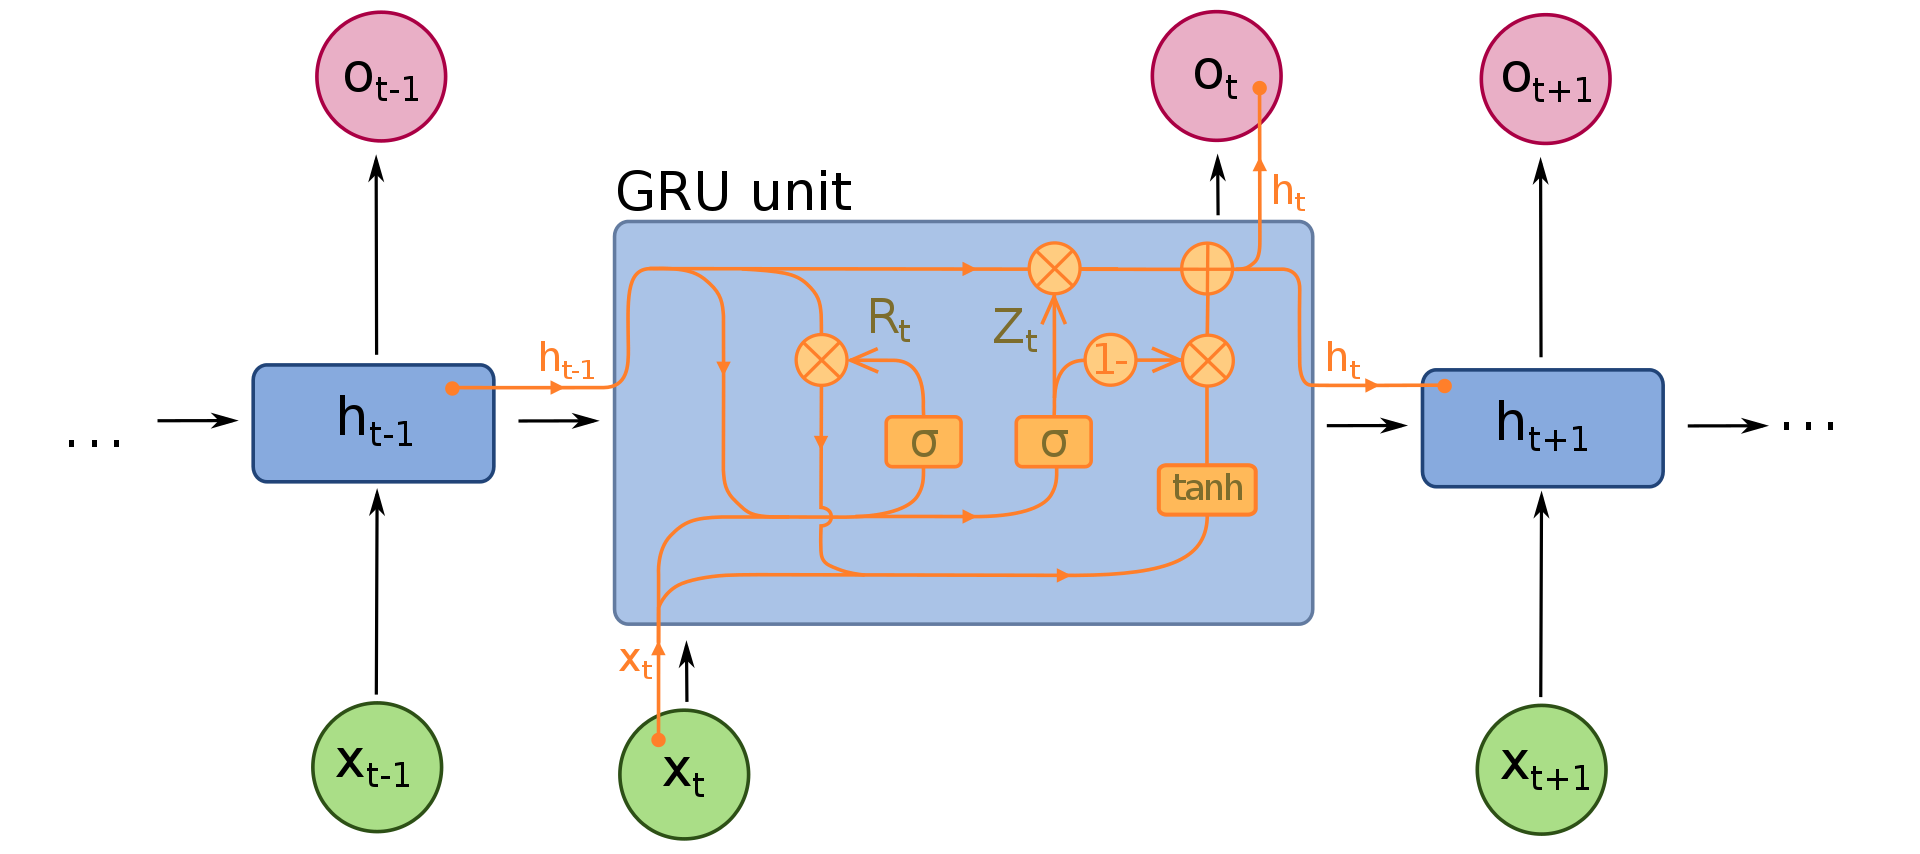
\includegraphics[width=14cm]{images/gru.png}
    \caption{A GRU cell}
    \label{fig:gru_cell}
\end{figure}

The different parameters are thus computed as follows\footnote{Biases $b$ removed for simplicity}:
\begin{align*}
        R_t &= \sigma\Big [ W_{ir} \bm{x}_t + W_{hr} \bm{h}_{t-1} \Big ] \\
        Z_t &= \sigma \Big [ W_{iz} \bm{x}_t + W_{hz} \bm{h}_{t-1} \Big ] \\
        \bm{n}_t &= \tanh \Big [ W_{in} \bm{x}_t + R_t \otimes W_{hz} \bm{h}_{t-1} \Big ] \\
        \bm{h}_t &= \big ( 1-Z_t \big ) \otimes \bm{n}_t + Z_t \otimes \bm{h}_{t-1} \\
\end{align*}
where $\otimes$ is an element-wise product. All the parameters $W_{xx}$ of the linear combinations have to be learned by applying SGD and backpropagation to a loss function defined over the outputs. Implementing all this is a non-trivial task but is greatly facilitated by the existence of deep learning frameworks.\\
While the defining characteristics of neural networks have been known since the 1980s, it was the combination of larger datasets, more computing power and new engineering techniques that led to the deep learning boom. In addition, several deep learning frameworks have been created to speed up development. These frameworks allow easy (and often dynamic) construction of computational graphs (roughly the architecture of the neural network) and implement automatically the backpropagation algorithm for the specific network. The best known frameworks are {\tt Tensorflow} (by Google), {\tt PyTorch} (by Facebook) and {\tt CNTK} (by Microsoft). In this work {\tt PyTorch} will be used.

%-----------------------------------------------------------------------------------------------
\subsection{Deep Q-Networks}
\label{sec:deep_qn}
A deep Q-network (DQN) was one of the first implementations of RL with deep learning methods. It's first use was to discover policies to play Atari games \cite{mnih2013playing} and is considered to be one of the breakthroughs of recent AI.\\
In DQN, a neural network is trained to estimate the $Q$-value of a particular state-action pair. This means that in algorithm \ref{algo:q_learning} the $Q(S,A)$ table is replaced with a neural net $f_{\theta}(S)$ that has $N_A$ outputs and thus  produces the estimated $Q$-value for each action $A$. Applied to Atari games like Pong, the state of the environment, and thus the input of this neural network, is the image of the game projected on the computer screen. Consequently, the initial layers of the neural net are convolutional layers, while the final layers are fully connected layers to estimate the output values.\\
Training is done by generating samples through interaction with the environment. The error needed to adjust the network weights is the square of the temporal difference of the traditional Q-learning algorithm:
\begin{equation}
\mathcal{L} = \big [y_t - Q(S_t, A_t); \theta \big ]^2
\label{eq:deep_Q_update}
\end{equation}
where $y_i$ is the target value, namely the best estimated Q-value reachable from the next state $S_{i+1}$, just as before:
\begin{equation}
y_t = R_t + \gamma \max_{A'} Q(S_{t+1}, A';\, \bm{\theta})
\label{eq:deep_Q_target}
\end{equation}
One of the problems with this setup is that machine learning techniques require that the samples that are used to learn from are independent and identically distributed (i.i.d.). Since the samples generated in the above way are part of the same trajectory, they are not independent. That's why the authors of \cite{mnih2015human} implement a \emph{replay memory} $D$: all samples are pooled and minibatches are sampled from this pool to perform learning. This avoids instabilities due to non-i.i.d. samples.\\
Another trick to improve the stability of learning is the use of a \emph{target network}  $\hat{Q}$ \cite{mnih2015human}, a copy of the action-value network that is used to compute the Q-value in the temporal difference value of equation \ref{eq:deep_Q_target}. This network is synchronized with the main network every $C$ steps. In this way, we avoid computing the target Q-value with the same network that gets updated during every iteration step. The DQN-algorithm is shown in algorithm \ref{algo:deep_q}. \\
Note here the procedure for action selection: the best action according to equation \ref{eq:optimal_policy} is not always selected; sometimes (more exactly, with probability $\epsilon$) an action is chosen randomly from the action-space. This action selection improves the exploration of the state-space and is called \emph{$\epsilon$-greedy}. The value of $\epsilon$ is reduced during learning, to shift from an emphasis on exploration of the state-action space to exploitation of promising results. The tension between exploration and exploitation is a classic trade-off in reinforcement learning.

\begin{algorithm}[H]
\SetAlgoLined
Initialize replay memory $D$ to capacity $N$\\
Initialize action-value function $Q$ with random weights $\bm{\theta}$\\
Initialize target action-value function $\hat{Q}$ with random weights $\bm{\theta}^- = \bm{\theta}$\\
\For{episode = 1\ldots M}{
    Initialize sequence $s_1 = \{x_1\}$
    \For{t=1\ldots }{
        With probability $\epsilon$, select a random action $a_t$\\
        Otherwise select $a_t = \argmax_{a}Q(s_t, a; \bm{\theta})$\\
        Execute action $a_t$ and observe reward $r_t$ and next state $s_{t+1}$\\
        Store tuple $(s_t, a_t, r_t, s_{t+1})$ in $D$\\
        Sample a random minibatch of transitions $(s_t, a_t, r_t, s_{t+1})$ from $D$.\\
        If episode terminates at step $j+1$, set $y_j = r_j$\\
        Otherwise, set $y_j = r_j + \gamma \max_{a'} Q(s_{j+1}, a'; \bm{\theta}^-)$\\
        Perform gradient descent step on $\Big  ( y_j - Q(s_j, a_j; \bm{\theta}) \Big )^2$\\
        Every $C$ steps, synchronize $\hat{Q} = Q$
    }
}
 \caption{Deep Q-learning with experience replay}
 \label{algo:deep_q}
\end{algorithm}

%----------------------------------------------------------------------------
\subsection{Deep Policy Gradients}
\label{sec:deep_pg}
When applying deep learning methods to the policy gradient methods of section \ref{sec:intro_policy_grads}, the policy that is to be optimized is represented as a neural network (see figure \ref{fig:deep_pg}). The input of the network is the system state (or observation) while the output is a distribution over the possible actions. The action to take is then sampled from this distribution.
\begin{figure}[htp]
    \centering
    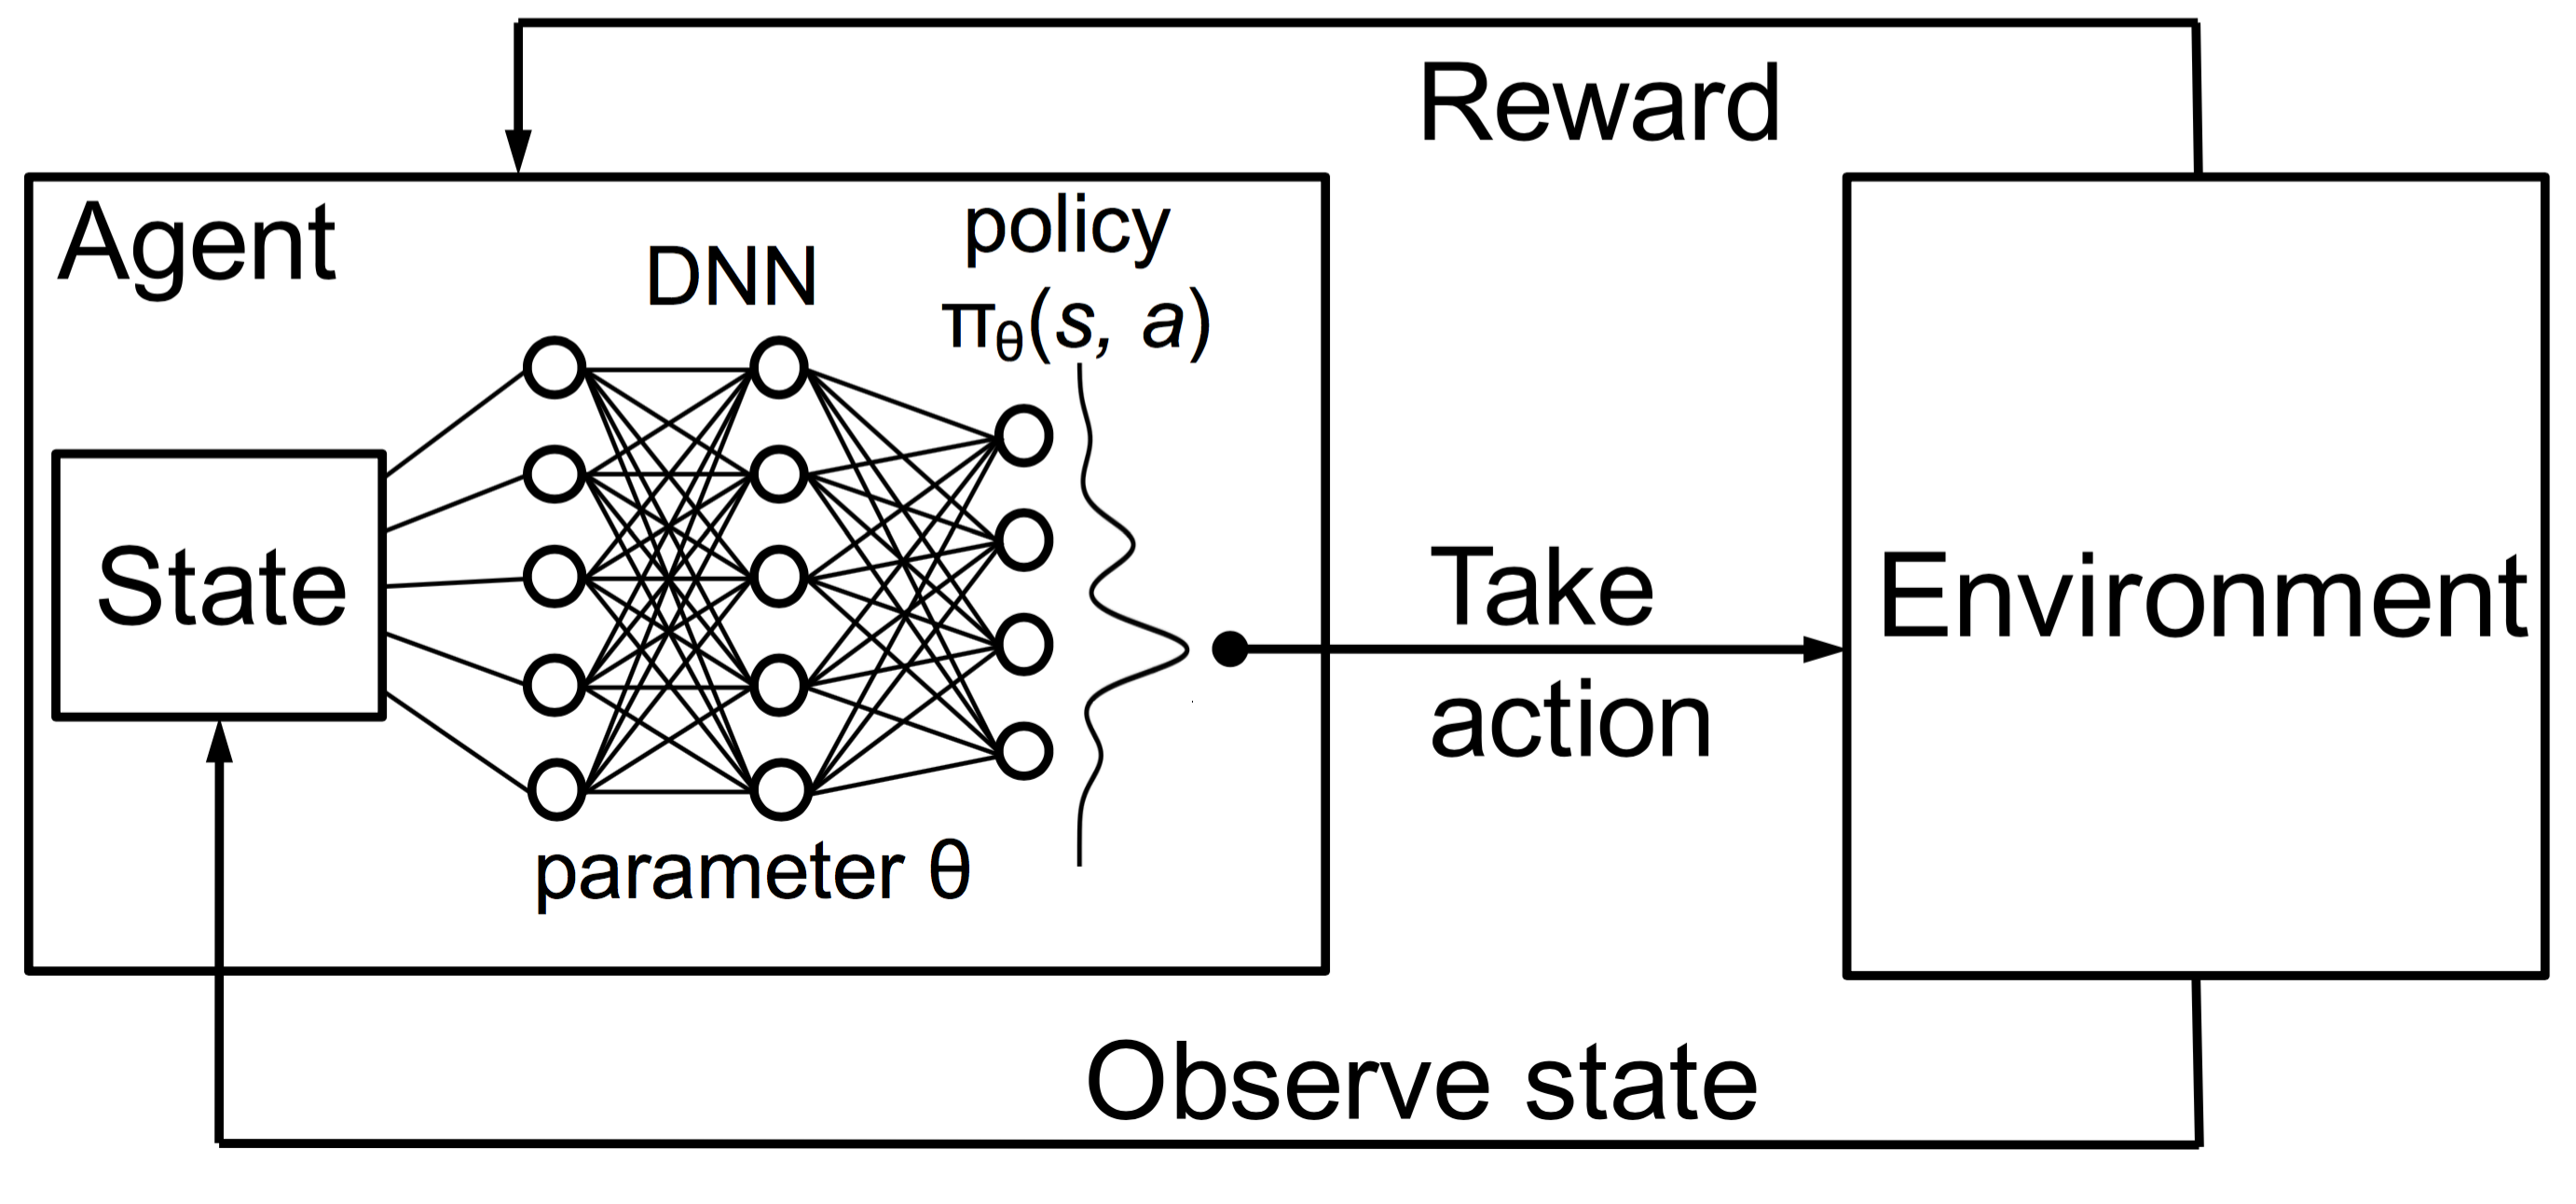
\includegraphics[width=10cm]{images/deep_pg.png}
    \caption{Deep Policy Gradient}
    \label{fig:deep_pg}
\end{figure}
Adjusting the network weights is done by using an update rule similar to equation \ref{eqn:pg_update}. The cost function thus becomes the logarithm over the action distribution.\\

Similarly, the critic will also be represented as a neural network. Typically, both actor- and critic-network share the lower layers in a common body, since they both have to process the same state and there is no reason to assume that the learned features in these layers should be different for actor or critic. This helps by letting actor and critic share the low-level features but combine them in a different way. The end result is a shared network which predicts action distributions and state values simultaneously. Learning is done more efficiently in this manner. Figure \ref{fig:common_body} represents this concept.

\begin{figure}[htp]
    \centering
    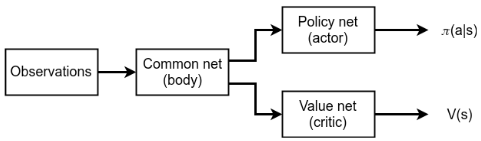
\includegraphics[width=12cm]{images/common_body.png}
    \caption{An actor-critic network with common body and separate heads}
    \label{fig:common_body}
\end{figure}

Just as in DQN, there is a high probability that an agent will converge to a policy that is locally optimal but is far from the global optimum. In other words, the policy space wasn't explored enough. In DQN, this can be solved by gradually decreasing the $\epsilon$-parameter in $\epsilon$-greedy action selection. While similar methods can be used for DPG, a better method is available. By adding the \emph{entropy}\footnote{The entropy of a probability distribution equals $H(\pi) = -\sum_{a} \pi(a|s) \log \pi(a|s)$. It is maximum when $\pi$ is uniform and minimal when all probability mass is placed on a single action.} $H(\pi)$ to the loss-function, we can penalize policies where the agent is too sure of certain actions, effectively steering the agent to policies that improve exploration of the policy space.\\
In the computational graph of a network of type \ref{fig:common_body}, we define only a single loss function and a single optimizer that will use this loss function to update the different weights. The loss function thus becomes the sum of three parts:
\begin{itemize}
    \item a term to simulate the step in the direction of an improved policy:\\ \begin{equation} \mathcal{L}_{pol} = -\log(A_t|S_t) \mathcal{A}(S_t, A_t) \end{equation} Mind the minus sign because we want to increase the value of the policy as the loss is minimized.
    \item a term to make the critic converge to a correct estimate of the value of the states:\\
    \begin{equation} \mathcal{L}_{val} =  \frac{1}{2} \big[ R_t + \gamma \max_{A'} Q(S_{t+1}, A') - Q(S_t, A_t)\big]^2 \end{equation} 
    \item a term that represents a fraction of the policy entropy, computed over all the states:\\ \begin{equation} \mathcal{L}_{ent} = -\beta H(s)\end{equation} 
\end{itemize}
The total loss is the combination of these three loss functions:
\begin{equation}
\mathcal{L} = \mathcal{L}_{pol} + \mathcal{L}_{val} + \mathcal{L}_{ent} 
\end{equation} 

The policies in the preceding paragraphs were conditioned on the current state $S_t$. The expressive power of these policy networks increases when we could condition on the entire set of previously seen observations, namely the state trajectory $\tau$. This is done implicitly by using recurrent networks like a GRU, where the hidden state encodes the information about the previously seen states. This is common practice in algorithms like COMA and QMix (see sections \ref{sec:intro_coma} and \ref{sec:intro_qmix}).
%----------------------------------------------------------------------------
\section{Multi-Agent Reinforcement Learning}
\label{sec:intro_marl}
While reinforcement learning is a promising technique for training agents, the mathematical framework that justifies it is inappropriate for multi-agent environments. The theory of Markov Decision Processes assumes that the agent's environment is stationary and no other adaptive agents are present. This is no longer the case when we consider multiple learning agents.\\

\emph{Markov Games} \cite{littman1994markov} are an extension of the MDP framework that accounts for interacting agents. To describe a Markov game with $k$ agents, we consider:
\begin{itemize}
    \item a set of states $\mathcal{S}$,
    \item a collection of action sets $A_1, \ldots, A_k$, one set for each agent,
\end{itemize}
Transitions from one state to the next are controlled by a transition function $T: \mathcal{S} \times A_1 \times \ldots A_k \rightarrow \text{PD}(\mathcal{S})$ with $\text{PD}(\mathcal{S})$ the set of probability distribution over states. It is important to note that a transition is determined by the \emph{joint action set} $A_1 \times \ldots A_k$ and not just a single action. Agents can thus influence each other in complex ways. A single instance of this joint action space is abbreviated $\bm{u} \in \mathcal{A} = A_1 \times \ldots A_k$. \\

Every agent $i$ has an associated reward function $\mathcal{R}_i: \mathcal{S} \times A_1 \times \ldots A_k \rightarrow \mathbb{R}$ and tries to maximize its expected sum of discounted rewards $\mathbb{E}\Big [ \sum_{j=0}^{\infty} \gamma^j R_{i, t+j} \Big ]$. Thus, since the rewards and transition function depends on the joint action set, the value and action-value functions for agent $i$ do as well:
\begin{equation}
    V_i^{\pi} = \sum_{\bm{u}}\pi(s, \bm{u}) \sum_{s} \mathcal{T}(s, u_i, \bm{u}_{-i}, s') \big [\mathcal{R}_i((s, u_i, \bm{u}_{-i}) + \gamma V_i(s')]
\end{equation}
and the optimal policy for agent $i$ will also depend on the policies of the other agents. This is another way of saying that in the presence of other learning agents, the environment isn't stationary.\\

The following sections describe a couple algorithms that try to maximize this term in an efficient manner. These algorithms are typically classified under the header of \emph{Multi-Agent Reinforcement Learning} (MARL).
A particular issue with multi-agent learning is the challenge of multi-agent \emph{credit assignment}: when two or more agents cooperate, which action of which agent led to the victory (or the loss)? Since the reward is global and the same for both players, this can be difficult to discern.
%----------------------------------------------------------------------------
\subsection{Independent Multi-Agent Learning}
\label{sec:intro_deep_indep_rl}
The simplest MARL algorithm, Independent Q-Learning (IQL) \cite{tan1993multi} simply ignores the multi-agent setting, and lets each learning agent $i$ train an state-action value function $Q_i(s, a_i)$ independently of the other agents. As such, this is just a simple extension of single-agent learning. Multiple agents always outperform a single agent because they have more resources and a better chance for receiving rewards. However, the true advantage from a multi-agent setting comes from cooperation between agents, something that is not addressed with this method. More implementation details on how the training of a set of agents with Independent Q-Learning is done can be found in appendix \ref{app:iql}.\\
Another algorithm along the same line is Independent Actor Critic (IAC), where the agents are trained independently with a DPG algorithm like REINFORCE or A2C. Both IQL and IAC have been implemented as part of this thesis. The goal is to provide a baseline against which other algorithms can be compared.

%----------------------------------------------------------------------------
%\subsection{Minimax Q-learning}
%\label{sec:intro_minimax_q}

%----------------------------------------------------------------------------
\subsection{QMIX}
\label{sec:intro_qmix}

\emph{QMIX} \cite{rashid2018qmix} is recent MARL algorithm that relies on the DQN paradigm. Properly capturing the effect's of the agents' actions requires a global action-value function $Q_{tot}(s, \bm{u})$. However,  this function is difficult to learn and even if learned, it is not obvious how to extract decentralized policies for individual agents. A simple solution would be to learn a centralised $Q_{tot}$ that is the sum of individual value functions $Q_i$ for the individual agents $i$:
\begin{equation}
    Q_{tot}(s, \bm{u}) = \sum_{i=1}^{n} Q_i(s_i, a_i)
\end{equation}
A decentralised policy for agent $i$ would then simply be greedy action selection based on $Q_i$. This is how \emph{Value Decomposition Networks} \cite{sunehag2018value} work. However, restraining $Q_{tot}$ to the sum of individual $Q$-functions is too restrictive.\\

The idea behind QMIX is that we only need to ensure that finding the best global joint action on $Q_{tot}$ yields the same result as a set of best actions on individual $Q_i$'s:
\begin{equation}
    \bm{u}^* = \argmax_{\bm{u}} Q_{tot}(s, \bm{u}) = \big [ \argmax_{a_1} Q_1(s, a_1), \, \ldots,\, \argmax_{a_N} Q_1(s, a_N) \big ]
\end{equation}
A sufficient condition to realize this is to enforce a monotonicity constraint on the relationship between $Q_{tot}$ and each $Q_i$:
\begin{equation}
    \label{eqn:qmix}
    \frac{\partial Q_{tot}}{\partial Q_i} \geq 0, \forall i
\end{equation}
QMIX does this by representing each $ Q_i$ by an \emph{agent network}. All these $Q_i$'s are combined into $Q_{tot}$ with a \emph{mixing network} in a non-linear way (contrary to VDN) but enforces conditions \ref{eqn:qmix} by forcing the weights of the mixing network to be positive. The details of these networks and how they interact is shown in figure \ref{fig:qmix_structure}.\\

\begin{figure}[htp]
    \centering
    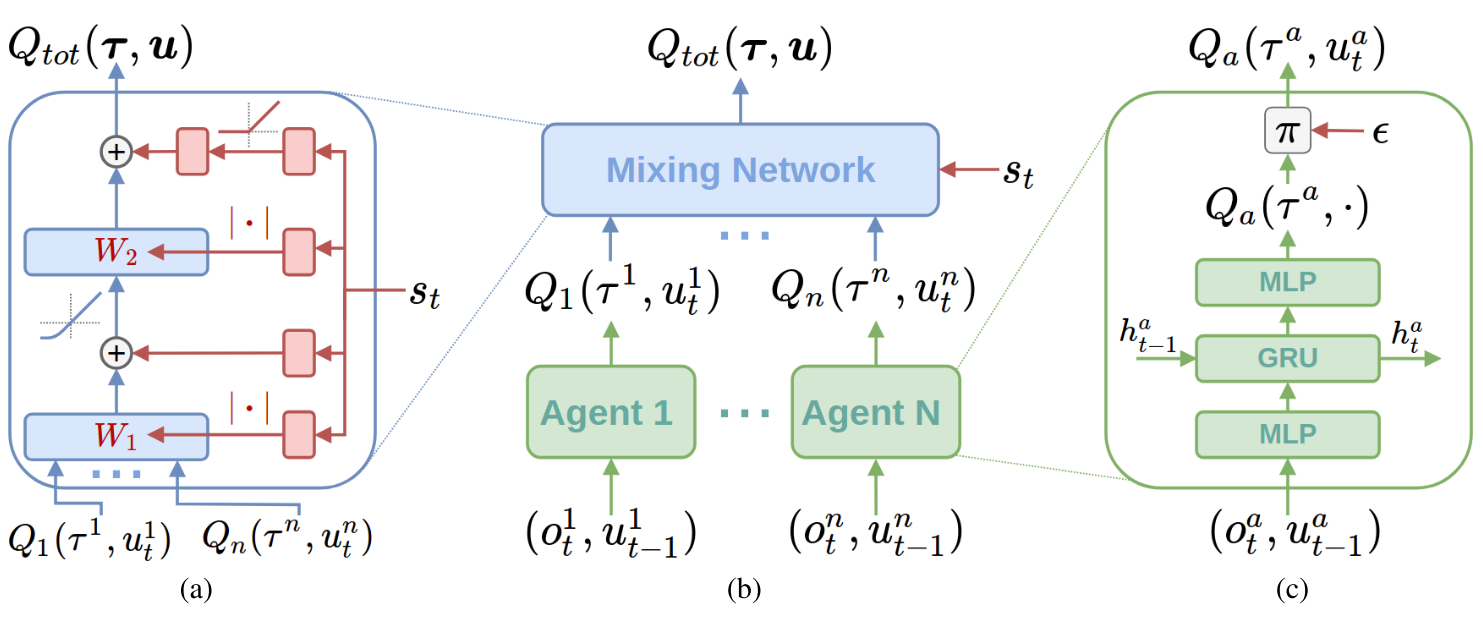
\includegraphics[width=16cm]{images/qmix_structure.png}
    \caption{Structure of QMIX (reproduced from \cite{rashid2018qmix})}
    \label{fig:qmix_structure}
\end{figure}

Figure (b) is the global structure, where the results of several agent networks are combined in a mixing network. Figure (c) shows an agent network. Once again, a recurrent net (a GRU) is used to track the agent's trajectory. The result is the "best" Q-value available in this state, determined by $\epsilon$-greedy selection. Figure (a) shows the mixing network. Small hypernetworks (in red) take the state $s$ and produce the weights $W_k$ of the network. They consists of a single linear layer and an absolute activation function $|\cdot|$ which ensures that these weights are always positive.

%----------------------------------------------------------------------------
\subsection{COMA}
\label{sec:intro_coma}
\emph{Counterfactual Multi-Agent Policy Gradients} (COMA) \cite{foerster2018counterfactual} is a recent multi-agent reinforcement learning algorithm based on actor-critic policy gradients. It uses the philosophy of \emph{centralised training of decentralised policies}, a multi-agent paradigm introduced by \cite{oliehoek2008optimal}. A decentralised policy is a policy in which each agent selects its own action based only on its local action-observation history. There is thus no way to coordinate any action with a team mate. This is a realistic point-of-view for our purposes, since we can assume that in critical situations, there will be no time for tanks to coordinate their actions. However, since learning the policies is done in a simulator, it is possible to use the entire state-space, including knowledge about teammates and their previous actions, to learn a strategy.\\

%The general concept of centralised learning - decentralised execution is represented in figure \ref{fig:central_decentral}, where training (in green) relies on critics who have access to the full state information, but who are no longer available during execution (in red).
%\begin{figure}[htp]
%    \centering
%    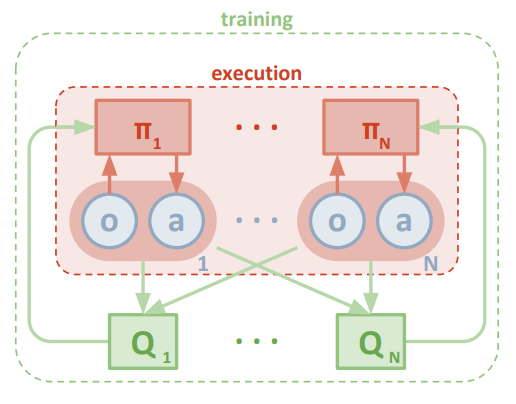
\includegraphics[width=10cm]{images/central_decentral.png}
%    \caption{Generic structure of centralised learning - decentralised execution}
%    \label{fig:central_decentral}
%\end{figure}
COMA trains a centralised critic, which is only used during learning. The actor, on the other hand, is trained during learning and used during execution. The critic conditions on the joint action space and all available state information, while each agent's policy conditions only on its own action-observation.\\

Another idea of COMA is to use a \emph{counterfactual baseline} to address the problem of credit assignment. COMA uses the centralised critic to compute a specific \emph{advantage function} for each agent. This function compares the estimated return of the current joint action to a counterfactual baseline that marginalizes out a single agent's action, while keeping the other agent's actions fixed \cite{foerster2018counterfactual}. The advantage for agent $i$ with policy $\pi^{i}$ is computed as:
\begin{equation}
    \label{eqn:coma}
    A^i(s, \bm{u}) = Q(s, \bm{u}) - \sum_{u^{'i}} \pi^{i}(u^{'i}|\tau^i) Q(s, (\bm{u}^{-i}, u^{'i}))
\end{equation}
where $\bm{u}^{-i}$ is shorthand for elements of the joint action space excluding the actions of agent $i$. In this expression, $Q(s, \bm{u})$ is the centralised critic that estimates $Q$-values for the joint action $\bm{u}$ conditioned on the central state $s$.\\
Thirdly, the critic representation that COMA uses to compute this counterfactual baseline is such that the computation can be done efficiently. All Q-values for all agents are computed in a single batched forward pass.\\
How all this is done is shown in figure \ref{fig:coma_structure}. Figure (a) shows how the agents interact with the environment through their actor, by applying actions $u_t^i$ and receiving observations $o_t^i$. At the same time, the actors inform the critic about their chosen action, while the critic returns the advantage value $A_t^i$. The red arrows and components are only required during the centralised learning.\\

\begin{figure}[htp]
    \centering
    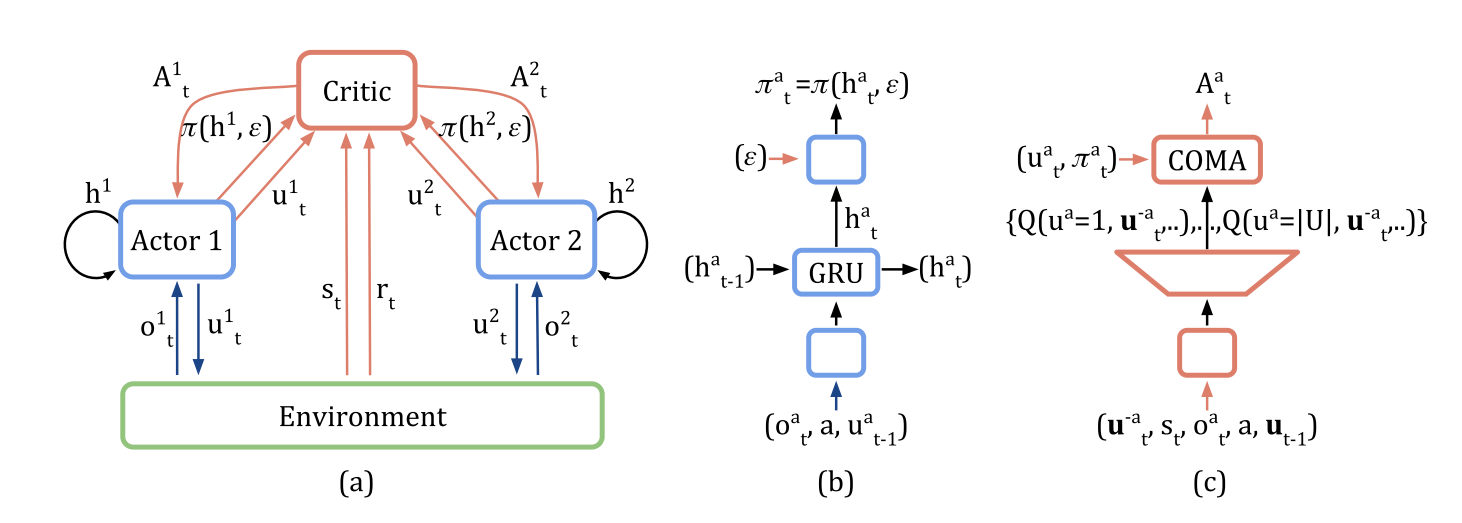
\includegraphics[width=16cm]{images/coma_structure.png}
    \caption{Structure of COMA (reproduced from \cite{foerster2018counterfactual})}
    \label{fig:coma_structure}
\end{figure}

Figure (b) shows the internal structure of the Actor. The Actor is a GRU, a specific instance of a recurrent network (see section \ref{sec:deep_learning}). The advantage of using a RNN in this context is that the action selection is based not only on the current observation, but also (albeit implicitly) on previous observations and actions. This corresponds to conditioning on the entire trajectory $\tau^i$ of the agent, a term that is also present in equation \ref{eqn:coma}.\\

The Critic (figure (c)) takes as input not only the observation $o_t^i$ and the agent's action $a$, but also the complete state information $s_t$ and the previous actions $\bm{u}_{t-1}$ and especially the actions of other agents $\bm{u}_t^{-i}$ at time $t$. The output is list of $Q$-values, one for each of the agent's actions $a$: $\{Q(u^i=1, \bm{u}_t^{-i}) \ldots  Q(u^i=|U|, \bm{u}_t^{-i}) \}$ with $|U|$ the size of the action space. Once these values are available, the counterfactual advantage $A^i(s, \bm{u})$ can thus be efficiently computed with expression \ref{eqn:coma}.

